% Options for packages loaded elsewhere
\PassOptionsToPackage{unicode}{hyperref}
\PassOptionsToPackage{hyphens}{url}
\PassOptionsToPackage{dvipsnames,svgnames,x11names}{xcolor}
%
\documentclass[
  letterpaper,
  DIV=11,
  numbers=noendperiod]{scrreprt}

\usepackage{amsmath,amssymb}
\usepackage{lmodern}
\usepackage{iftex}
\ifPDFTeX
  \usepackage[T1]{fontenc}
  \usepackage[utf8]{inputenc}
  \usepackage{textcomp} % provide euro and other symbols
\else % if luatex or xetex
  \usepackage{unicode-math}
  \defaultfontfeatures{Scale=MatchLowercase}
  \defaultfontfeatures[\rmfamily]{Ligatures=TeX,Scale=1}
\fi
% Use upquote if available, for straight quotes in verbatim environments
\IfFileExists{upquote.sty}{\usepackage{upquote}}{}
\IfFileExists{microtype.sty}{% use microtype if available
  \usepackage[]{microtype}
  \UseMicrotypeSet[protrusion]{basicmath} % disable protrusion for tt fonts
}{}
\makeatletter
\@ifundefined{KOMAClassName}{% if non-KOMA class
  \IfFileExists{parskip.sty}{%
    \usepackage{parskip}
  }{% else
    \setlength{\parindent}{0pt}
    \setlength{\parskip}{6pt plus 2pt minus 1pt}}
}{% if KOMA class
  \KOMAoptions{parskip=half}}
\makeatother
\usepackage{xcolor}
\usepackage[normalem]{ulem}
\setlength{\emergencystretch}{3em} % prevent overfull lines
\setcounter{secnumdepth}{1}
% Make \paragraph and \subparagraph free-standing
\ifx\paragraph\undefined\else
  \let\oldparagraph\paragraph
  \renewcommand{\paragraph}[1]{\oldparagraph{#1}\mbox{}}
\fi
\ifx\subparagraph\undefined\else
  \let\oldsubparagraph\subparagraph
  \renewcommand{\subparagraph}[1]{\oldsubparagraph{#1}\mbox{}}
\fi


\providecommand{\tightlist}{%
  \setlength{\itemsep}{0pt}\setlength{\parskip}{0pt}}\usepackage{longtable,booktabs,array}
\usepackage{calc} % for calculating minipage widths
% Correct order of tables after \paragraph or \subparagraph
\usepackage{etoolbox}
\makeatletter
\patchcmd\longtable{\par}{\if@noskipsec\mbox{}\fi\par}{}{}
\makeatother
% Allow footnotes in longtable head/foot
\IfFileExists{footnotehyper.sty}{\usepackage{footnotehyper}}{\usepackage{footnote}}
\makesavenoteenv{longtable}
\usepackage{graphicx}
\makeatletter
\def\maxwidth{\ifdim\Gin@nat@width>\linewidth\linewidth\else\Gin@nat@width\fi}
\def\maxheight{\ifdim\Gin@nat@height>\textheight\textheight\else\Gin@nat@height\fi}
\makeatother
% Scale images if necessary, so that they will not overflow the page
% margins by default, and it is still possible to overwrite the defaults
% using explicit options in \includegraphics[width, height, ...]{}
\setkeys{Gin}{width=\maxwidth,height=\maxheight,keepaspectratio}
% Set default figure placement to htbp
\makeatletter
\def\fps@figure{htbp}
\makeatother
\newlength{\cslhangindent}
\setlength{\cslhangindent}{1.5em}
\newlength{\csllabelwidth}
\setlength{\csllabelwidth}{3em}
\newlength{\cslentryspacingunit} % times entry-spacing
\setlength{\cslentryspacingunit}{\parskip}
\newenvironment{CSLReferences}[2] % #1 hanging-ident, #2 entry spacing
 {% don't indent paragraphs
  \setlength{\parindent}{0pt}
  % turn on hanging indent if param 1 is 1
  \ifodd #1
  \let\oldpar\par
  \def\par{\hangindent=\cslhangindent\oldpar}
  \fi
  % set entry spacing
  \setlength{\parskip}{#2\cslentryspacingunit}
 }%
 {}
\usepackage{calc}
\newcommand{\CSLBlock}[1]{#1\hfill\break}
\newcommand{\CSLLeftMargin}[1]{\parbox[t]{\csllabelwidth}{#1}}
\newcommand{\CSLRightInline}[1]{\parbox[t]{\linewidth - \csllabelwidth}{#1}\break}
\newcommand{\CSLIndent}[1]{\hspace{\cslhangindent}#1}

\KOMAoption{captions}{tableheading}
\makeatletter
\makeatother
\makeatletter
\@ifpackageloaded{bookmark}{}{\usepackage{bookmark}}
\makeatother
\makeatletter
\@ifpackageloaded{caption}{}{\usepackage{caption}}
\AtBeginDocument{%
\ifdefined\contentsname
  \renewcommand*\contentsname{Table of contents}
\else
  \newcommand\contentsname{Table of contents}
\fi
\ifdefined\listfigurename
  \renewcommand*\listfigurename{List of Figures}
\else
  \newcommand\listfigurename{List of Figures}
\fi
\ifdefined\listtablename
  \renewcommand*\listtablename{List of Tables}
\else
  \newcommand\listtablename{List of Tables}
\fi
\ifdefined\figurename
  \renewcommand*\figurename{Figure}
\else
  \newcommand\figurename{Figure}
\fi
\ifdefined\tablename
  \renewcommand*\tablename{Table}
\else
  \newcommand\tablename{Table}
\fi
}
\@ifpackageloaded{float}{}{\usepackage{float}}
\floatstyle{ruled}
\@ifundefined{c@chapter}{\newfloat{codelisting}{h}{lop}}{\newfloat{codelisting}{h}{lop}[chapter]}
\floatname{codelisting}{Listing}
\newcommand*\listoflistings{\listof{codelisting}{List of Listings}}
\makeatother
\makeatletter
\@ifpackageloaded{caption}{}{\usepackage{caption}}
\@ifpackageloaded{subcaption}{}{\usepackage{subcaption}}
\makeatother
\makeatletter
\@ifpackageloaded{tcolorbox}{}{\usepackage[many]{tcolorbox}}
\makeatother
\makeatletter
\@ifundefined{shadecolor}{\definecolor{shadecolor}{rgb}{.97, .97, .97}}
\makeatother
\makeatletter
\makeatother
\ifLuaTeX
  \usepackage{selnolig}  % disable illegal ligatures
\fi
\IfFileExists{bookmark.sty}{\usepackage{bookmark}}{\usepackage{hyperref}}
\IfFileExists{xurl.sty}{\usepackage{xurl}}{} % add URL line breaks if available
\urlstyle{same} % disable monospaced font for URLs
\hypersetup{
  pdftitle={Autism All Grown Up},
  pdfauthor={Ariel Balter},
  colorlinks=true,
  linkcolor={blue},
  filecolor={Maroon},
  citecolor={Blue},
  urlcolor={Blue},
  pdfcreator={LaTeX via pandoc}}

\title{Autism All Grown Up}
\usepackage{etoolbox}
\makeatletter
\providecommand{\subtitle}[1]{% add subtitle to \maketitle
  \apptocmd{\@title}{\par {\large #1 \par}}{}{}
}
\makeatother
\subtitle{The Autism Nexus of Oregon}
\author{Ariel Balter}
\date{6/4/24}

\begin{document}
\maketitle
\ifdefined\Shaded\renewenvironment{Shaded}{\begin{tcolorbox}[breakable, frame hidden, borderline west={3pt}{0pt}{shadecolor}, interior hidden, sharp corners, enhanced, boxrule=0pt]}{\end{tcolorbox}}\fi

\renewcommand*\contentsname{Contents}
{
\hypersetup{linkcolor=}
\setcounter{tocdepth}{1}
\tableofcontents
}
\bookmarksetup{startatroot}

\hypertarget{section}{%
\chapter{}\label{section}}


\includegraphics[width=3.09896in,height=3.05923in]{././media/image4.png}

\bookmarksetup{startatroot}

\hypertarget{sec-mission}{%
\chapter{Mission}\label{sec-mission}}

The mission of Autism All Grown Up (AAGU) is to empower autistic adults
in Oregon by serving as a nexus that provides accessible information,
resources, and services tailored to their unique needs. By bridging gaps
in the existing infrastructure, we connect and interconnect the adult
autistic community and their supporters, facilitate information
exchange, and promote collaboration. This ensures that autistic
individuals can access the support and opportunities they need to
thrive, enhancing their well-being and independence throughout the
state.

\bookmarksetup{startatroot}

\hypertarget{sec-executive_summary}{%
\chapter{Executive Summary}\label{sec-executive_summary}}

\hypertarget{sec-ex_sum_background}{%
\section{Background}\label{sec-ex_sum_background}}

Dr.~Ariel Balter, an experienced scientist and data analyst, was
diagnosed with ADHD and ASD later in life and is raising a teenager with
both diagnoses. His desire to understand these challenges led him to
study the scientific and social aspects of neurodiversity. Recent
changes driven by autistic self-advocates and researchers have reshaped
our understanding of autism, revealing significant gaps in support for
autistic adults. These changes have led to controversies and arguments
that are still unfolding, emphasizing the evolving nature of the
understanding of autism.

Through his personal journey and interactions with the local autistic
community, Dr.~Balter identified significant gaps in services, support,
and understanding for autistic adults without intellectual disabilities.
He was struck by the level of unmet need he heard from his
peers---people with skills, education, and abilities but struggling for
reasons related to autism. These personal experiences led Dr.~Balter to
found Autism All Grown Up (AAGU) to address these gaps.

\hypertarget{sec-ex_sum_goals}{%
\section{Goals}\label{sec-ex_sum_goals}}

The organization has four key objectives:

\begin{enumerate}
\def\labelenumi{\arabic{enumi}.}
\tightlist
\item
  Facilitate connections and collaboration within the adult autistic
  community
\item
  Identify the unmet needs of autistic adults and report on the causes
\item
  Provide accurate, accessible, and up-to-date information and resources
  \emph{for} autistic adults
\item
  Provide accurate, accessible, and up-to-date information and resources
  \emph{about} autism and \emph{about} the autistic community
\end{enumerate}

\hypertarget{sec-ex_name}{%
\section{Autism All Grown Up}\label{sec-ex_name}}

Autism is all grown up, and it isn't pretty. The phrase ``All Grown Up''
captures the bittersweet realization that often occurs when one
encounters an individual they knew as a child, only to find that their
preconceived notions no longer fit the adult standing before them.

For decades, autism was seen as a developmental challenge that primarily
affected children. Outdated notions of what constitutes genuine autism
have cause adults to be overlooked by many people. Because so little
research has acknowledged the lives of adults with autism, we know close
to nothing about what successful adult development looks like. Some
existing research suggests that autistic adults face reduced life
expectancy, increased risk for physical disability, and an earlier onset
of age-related cognitive concerns. Late-identified and never-identified
autistic adults face unique challenges with respect to aging, and most
of these ``lost generations'' (Wright 2015) have not yet even been
counted.

\hypertarget{sec-ex_sum_nexus}{%
\section{The Nexus Approach}\label{sec-ex_sum_nexus}}

Rather than working on advocacy, Dr.~Balter feels he can more directly
serve the autistic community in Oregon by solving problems on the
ground. Systemic and societal problems can only be addressed through
advocacy. But many of the real-world problems faced by supporting
existing infrastructure by increasing the connectivity and information
flow. Rather than being a hub that consumes resources and provides
services, AAGU will catalyze and strengthen relationships around it to
form a \emph{nexus}.

\bookmarksetup{startatroot}

\hypertarget{sec-autism2024}{%
\chapter{Autism in 2024}\label{sec-autism2024}}

\hypertarget{the-new-world-of-autism}{%
\section{The New World of Autism}\label{the-new-world-of-autism}}

Recent advancements in our understanding of autism, largely driven by
autistic self-advocates and researchers, have highlighted the need for a
paradigm shift in understanding and supporting autistic individuals. Key
findings include (\textbf{ASAN2009?},@Weiss2023):

\begin{itemize}
\item
  \textbf{The Autism Spectrum is not Linear}

  Autistic people aren't ``more'' or ``less'' autistic so much as they
  are autistic in different ways.
\end{itemize}

\begin{figure}

{\centering 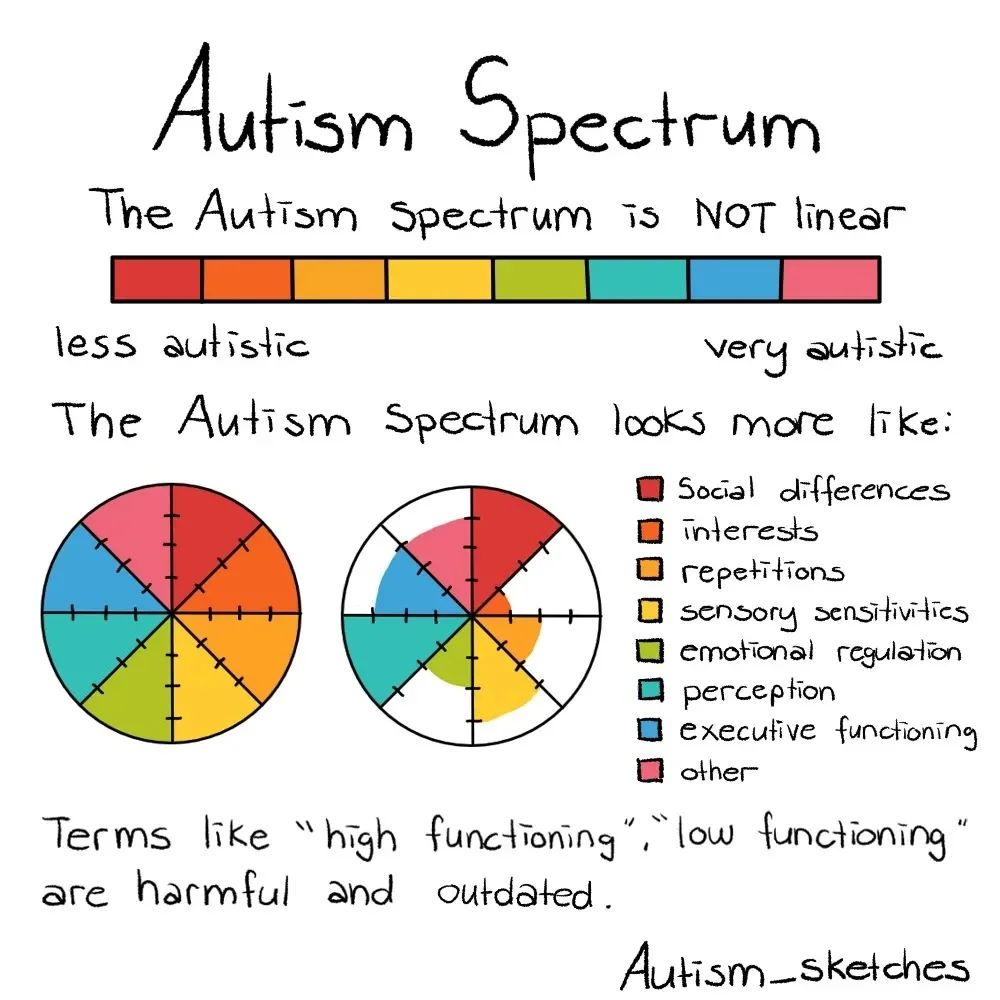
\includegraphics[width=0.5\textwidth,height=\textheight]{./media/autism_spectrum.jpeg}

}

\caption{Figure 1. What the autism spectrum means.}

\end{figure}

\begin{itemize}
\item
  \textbf{Disability can be Contextual:}

  Most autistic individuals are not intellectually or physically
  disabled but face substantial challenges navigating society.
  Navigating society feels like being a left-handed person using
  right-handed scissors: difficult and unwieldy at best.
\item
  \textbf{Misconceptions:}

  Science has refuted many harmful misconceptions about autism. Some
  autistic people have different accompanying conditions that can result
  in problems with body awareness, identifying their emotional state, or
  using speech. However, autistic people do not intrinsically lack
  feelings, empathy, social skills, or the ability to communicate.
\item
  \textbf{Lifelong Condition:}

  Autism is a lifelong neurological difference, not a disorder to be
  cured. There are roughly the same percentage of autistic adults as
  children, but there are four times as many adults as children.
\item
  \textbf{Neurodiversity \& Neurodivergence:}

  The \emph{neurodiversity paradigm} recognizes autism as a natural
  variation in human neurology. Individual people with cognitive styles
  that are significantly atypical are \emph{neurodivergent}, and many
  have unmet needs.
\end{itemize}

\hypertarget{sec-autism2024_lost_gen}{%
\section{Lost Generations of Autistic
Adults}\label{sec-autism2024_lost_gen}}

Autistic adults face unique challenges that are often overlooked, such
as navigating social and employment environments not designed for
neurodivergent individuals. Autistic adults without intellectual
disabilities often face a lack of access to appropriate healthcare and
support services.

Autistic adults perceived as having lower support needs face a
conundrum. While they rarely qualify for existing systems of support,
most face significant challenges that are often overlooked, dismissed,
or disbelieved. Most autistic people will tell you that the hardest part
about being autistic isn't being autistic but navigating a neurotypical
world that includes unconscious bias and ableism. Research backs this
up, indicating that discrimination, not autism, is a significant barrier
in the workplace.

Autistic adults face unique challenges that are often overlooked, such
as navigating social and employment environments not designed for
neurodivergent individuals. Key issues include:

\begin{itemize}
\tightlist
\item
  \textbf{Focus Gaps:} Research and services have predominantly focused
  on children leaving out adults, especially those without profound
  disabilities. We have failed, and continue to fail, to adequately
  study autistic life after high school when children lose many
  supports.
\end{itemize}

Despite these challenges, many autistic adults possess valuable skills,
talents, and perspectives that society misses out on by not
acknowledging their needs, hearing their voices, and making room for
them at the table.

\bookmarksetup{startatroot}

\hypertarget{sec-aagu}{%
\chapter{Autism All Grown Up (AAGU): A Nexus for
Change}\label{sec-aagu}}

\hypertarget{sec-aagu_origin}{%
\section{Origin}\label{sec-aagu_origin}}

AAGU was born out of Dr.~Balter's desire to use his personal experiences
and analytical skills to help his newfound community. By conducting root
cause analyses and working with local organizations, he identified key
areas where AAGU could make an immediate impact, such as:

\begin{itemize}
\tightlist
\item
  Creating accessible guides for obtaining adult autism diagnoses
  through Oregon's Medicaid and Vocational Rehabilitation systems
\item
  Establishing The Uncommons, autism-friendly co-working and community
  spaces
\item
  Improving online resources for autistic adults and providing
  consulting services to others to do the same
\item
  Participating in data analysis and research efforts to better
  understand the needs of autistic adults in Oregon
\end{itemize}

\hypertarget{sec-aagu_started}{%
\section{What We Have Started}\label{sec-aagu_started}}

AAGU has already made strides in achieving its objectives through
initiatives such as:

\begin{itemize}
\tightlist
\item
  Partnering with Health Share Oregon to create guides for accessing
  autism assessments through Medicaid and developing a template Letter
  of Medical Necessity to facilitate evaluations through I/DD and
  Vocational Rehab programs
\item
  Securing temporary spaces for The Uncommons, autism-friendly
  co-working and community spaces
\item
  Consulting with the Autism Society of Oregon to improve their online
  resources
\item
  Participating in the Oregon Commission on Autism Spectrum Disorder's
  data working group
\end{itemize}

\hypertarget{sec-aagu_goals}{%
\section{Goals}\label{sec-aagu_goals}}

Autism All Grown Up (AAGU) seeks to activate and empower the autistic
community in Oregon by improving communication channels and information
resources. Our immediate actions include:

\begin{itemize}
\tightlist
\item
  Establishing The Uncommons, a meeting and coworking space for autistic
  adults
\item
  Creating comprehensive guides on navigating healthcare, employment,
  and social services
\item
  Building partnerships with local organizations to enhance service
  delivery
\item
  Participating in data analysis and research to inform policy and
  advocacy efforts
\end{itemize}

Our growth plan consists of three phases:

\begin{enumerate}
\def\labelenumi{\arabic{enumi}.}
\tightlist
\item
  Seed (Weeks 1-8): Set up organizational structure, solicit initial
  funds, establish community presence, and build initial partnerships
\item
  Sprout (Weeks 9-26): Continue building community connections, develop
  The Uncommons, create informational materials, and identify large
  funding opportunities
\item
  Grow (Beyond Week 26): Expand The Uncommons, apply for large grants,
  build information and communication infrastructure, and establish a
  sustainable model for ongoing operations
\end{enumerate}

\hypertarget{sec-aagu_growth_plan}{%
\section{Growth Plan}\label{sec-aagu_growth_plan}}

Our growth plan consists of three phases:

\textbf{1. Seed (Weeks 1-8)}

\begin{itemize}
\tightlist
\item
  \textbf{Budget:} \$2,310/week
\item
  \textbf{Effort:} 1.5 FTE
\item
  \textbf{Actions:}

  \begin{itemize}
  \tightlist
  \item
    Set up organizational structure
  \item
    Solicit initial funds
  \item
    Establish community presence
  \item
    Build initial partnerships
  \end{itemize}
\end{itemize}

\textbf{2. Sprout (Weeks 9-26)}

\begin{itemize}
\tightlist
\item
  \textbf{Budget:} \$4,620/week
\item
  \textbf{Effort:} 2.75 FTE
\item
  \textbf{Actions:}

  \begin{itemize}
  \tightlist
  \item
    Continue building community connections
  \item
    Develop The Uncommons
  \item
    Create informational materials
  \item
    Identify large funding opportunities
  \end{itemize}
\end{itemize}

\textbf{3. Grow (Beyond Week 26)}

\begin{itemize}
\tightlist
\item
  \textbf{Budget:} \$6,468/week
\item
  \textbf{Effort:} 4.25 FTE
\item
  \textbf{Actions:}

  \begin{itemize}
  \tightlist
  \item
    Expand The Uncommons
  \item
    Apply for large grants
  \item
    Build information and communication infrastructure
  \item
    Establish a sustainable model for ongoing operations
  \end{itemize}
\end{itemize}

By establishing a comprehensive support system for autistic adults, AAGU
aims to improve their quality of life, promote independence, and foster
a sense of community and belonging. Through a phased growth plan, AAGU
will continue to expand its reach and impact, with a strong emphasis on
hiring autistic individuals and providing them with meaningful
employment opportunities. By leveraging the strengths and talents of the
autistic community, AAGU is uniquely positioned to create lasting,
positive change for autistic adults in Oregon.

\bookmarksetup{startatroot}

\hypertarget{funding}{%
\chapter{Funding}\label{funding}}

We are poised to launch a GoFundMe crowdsource campaign as soon as we
have our nonprofit status confirmed by ARRO. We hope to raise seed money
of \$2k-\$3k per week to jump start formal operations ************* next
\$34k for our 8-week Sprout phase. We hope to launch the Sprout phase
within our first month.

A key element of our first 8 weeks of formal operation (Sprout) will be
to create a calendar of funding deadlines and communicate with funders
to prioritize our initial grant-writing efforts. It will also be crucial
that we complete the initial projects we have started during the Sprout
phase to demonstrate our effectiveness to potential supporters. At the
end of the Sprout phase, we will report to our umbrella organizations
and all funders/sponsors.

We are on the verge of launching a GoFundMe crowdsource campaign, a
crucial step that hinges on our nonprofit status being confirmed by
ARRO. The urgency is palpable as we aim to raise a substantial seed fund
of \$2k-\$3k per week, a total of \$ 34k, to kickstart our formal
operations. This will pave the way for our 8-week Sprout phase, which we
plan to initiate within our first month.

Our initial 8 weeks of formal operation, known as the Sprout phase, are
meticulously planned. We will create a comprehensive calendar of funding
deadlines and engage in proactive communication with funders to
prioritize our grant-writing efforts. Equally important is the
completion of our initial projects during this phase, which will serve
as tangible proof of our effectiveness to potential supporters. At the
end of the Sprout phase, we will provide a detailed report to our
umbrella organizations and all funders/sponsors.

We have already identified almost 100 grants and sponsorships for which
we meet the basic requirements. These include grants from the State of
Oregon (e.g.~Oregon Health Authority), Oregon healthcare companies
(Legacy, Pacific Source, Cambia, etc.), and a mixture of private and
public foundations and trusts. We have missed the 2024 funding cycle for
some of these, but many have multiple cycles per year or do not run in
cycles. Some of these are small pots of money, and others regularly
award hundreds of thousands of dollars. We will also collect
sliding-scale fees for using \emph{The Uncommons} co-working spaces.

During our Grow phase, we hope to show that we can collect, analyze, and
disseminate information for and about the adult autistic community with
a very high level of capacity and efficiency. We hope this expertise
will enable us to secure outside contracts as subject matter experts,
analysts, and report writers, providing another avenue for revenue. We
will complete the Grow phase with a report to our umbrella organization
and our financial supporters.

\bookmarksetup{startatroot}

\hypertarget{budget}{%
\chapter{Budget}\label{budget}}

Autism All Grown Up will place a strong emphasis on hiring autistic and
neurodiverse Oregon adults and paying them a market wage. The wages will
be at the low end during the initial Seed and Sprout phases and increase
during the later phases. The hourly rates shown represent full
compensation on a 1099 and do not include benefits. We will make
necessary adjustments when we are able to provide benefits as well.

We have created our budget estimate based on the minimum staffing we
believe can meet our performance goals combined with market-rate salary
estimates from ZipRecruiter
(\href{https://www.ziprecruiter.com/Salaries}{\uline{https://www.ziprecruiter.com/Salaries}})
for approximate job titles in the Portland, OR area (see
\protect\hyperlink{appendix-2-representative-salaries}{\uline{Appendix
2: Representative Salaries}}). We project a budget of approximately
\$150,000 for the first six months (26 weeks) of operation.

\hypertarget{section-1}{%
\section{}\label{section-1}}

\hypertarget{seed}{%
\section{\texorpdfstring{\textbf{Seed}}{Seed}}\label{seed}}

\hypertarget{staffing}{%
\subsection{Staffing}\label{staffing}}

\begin{longtable}[]{@{}
  >{\raggedright\arraybackslash}p{(\columnwidth - 4\tabcolsep) * \real{0.1106}}
  >{\raggedright\arraybackslash}p{(\columnwidth - 4\tabcolsep) * \real{0.0426}}
  >{\raggedright\arraybackslash}p{(\columnwidth - 4\tabcolsep) * \real{0.8468}}@{}}
\toprule()
\begin{minipage}[b]{\linewidth}\raggedright
\textbf{Res ponsibility}
\end{minipage} & \begin{minipage}[b]{\linewidth}\raggedright
\textbf{FTE}
\end{minipage} & \begin{minipage}[b]{\linewidth}\raggedright
\textbf{Description}
\end{minipage} \\
\midrule()
\endhead
Organizing and Directing & 0.75 & Implement business systems--payrol,
formal job descriptions, insurance, etc. Hold regular meetings with
select partner organizations and individuals. Solicit and apply for
funding for Sprout phase. \\
Coworking space manager & 0.25 & Research how coworking spaces run.
Create a budget and game plan for initial set-up. Begin planning
marketing and promotion. \\
Research support & 0.25 & Collect and organize information. Writing. \\
Web Development & 0.25 & Design and build website. \\
\textbf{Total} & \textbf{1.50} & \\
\bottomrule()
\end{longtable}

\hypertarget{budget-1}{%
\subsection{Budget}\label{budget-1}}

\begin{longtable}[]{@{}
  >{\raggedright\arraybackslash}p{(\columnwidth - 8\tabcolsep) * \real{0.3133}}
  >{\raggedright\arraybackslash}p{(\columnwidth - 8\tabcolsep) * \real{0.1084}}
  >{\raggedright\arraybackslash}p{(\columnwidth - 8\tabcolsep) * \real{0.1205}}
  >{\raggedright\arraybackslash}p{(\columnwidth - 8\tabcolsep) * \real{0.2169}}
  >{\raggedright\arraybackslash}p{(\columnwidth - 8\tabcolsep) * \real{0.2410}}@{}}
\toprule()
\begin{minipage}[b]{\linewidth}\raggedright
\textbf{Respo nsibility}
\end{minipage} & \begin{minipage}[b]{\linewidth}\raggedright
\textbf{FTE}
\end{minipage} & \begin{minipage}[b]{\linewidth}\raggedright
\textbf{Rate}
\end{minipage} & \begin{minipage}[b]{\linewidth}\raggedright
\textbf{Weekly Total}
\end{minipage} & \begin{minipage}[b]{\linewidth}\raggedright
\textbf{Overhead (10\%)}
\end{minipage} \\
\midrule()
\endhead
Organizing and Directing & 0.75 & \$40.00 & \$1,200.00 & \$120.00 \\
Coworking space manager & 0.25 & \$30.00 & \$300.00 & \$30.00 \\
Research support & 0.25 & \$30.00 & \$300.00 & \$30.00 \\
Web Development & 0.25 & \$30.00 & \$300.00 & \$30.00 \\
Subtotal per week & & & \$2,100.00 & \$210.00 \\
\textbf{Total per week} & & & \textbf{\$ 2,310.00} & \\
\bottomrule()
\end{longtable}

\hypertarget{section-2}{%
\section{}\label{section-2}}

\hypertarget{section-3}{%
\section{}\label{section-3}}

\hypertarget{sprout}{%
\section{\texorpdfstring{\textbf{Sprout}}{Sprout}}\label{sprout}}

\hypertarget{staffing-1}{%
\subsection{\texorpdfstring{\textbf{Staffing}}{Staffing}}\label{staffing-1}}

\begin{longtable}[]{@{}
  >{\raggedright\arraybackslash}p{(\columnwidth - 4\tabcolsep) * \real{0.1057}}
  >{\raggedright\arraybackslash}p{(\columnwidth - 4\tabcolsep) * \real{0.0407}}
  >{\raggedright\arraybackslash}p{(\columnwidth - 4\tabcolsep) * \real{0.8537}}@{}}
\toprule()
\begin{minipage}[b]{\linewidth}\raggedright
\textbf{R esponsibility}
\end{minipage} & \begin{minipage}[b]{\linewidth}\raggedright
\textbf{FTE}
\end{minipage} & \begin{minipage}[b]{\linewidth}\raggedright
\textbf{Description}
\end{minipage} \\
\midrule()
\endhead
Organizing and Directing & 0.75 & Complete current information product
projects. Investigate access gaps. Locate resources. Continue building
relationships. Oversee and participate in research on community
resources and funding opportunities. \\
Data engineering & 0.50 & Create databases. Research portal design. \\
Coworking space manager & 0.50 & Research how coworking spaces run.
Solicit community feedback. Run trails. \\
Research support & 0.50 & Collect and organize information. Writing. \\
Web Development & 0.50 & Design and build website. \\
\textbf{Total} & \textbf{2.75} & \\
\bottomrule()
\end{longtable}

\hypertarget{budget-2}{%
\subsection{\texorpdfstring{\textbf{Budget}}{Budget}}\label{budget-2}}

\begin{longtable}[]{@{}
  >{\raggedright\arraybackslash}p{(\columnwidth - 8\tabcolsep) * \real{0.3133}}
  >{\raggedright\arraybackslash}p{(\columnwidth - 8\tabcolsep) * \real{0.1084}}
  >{\raggedright\arraybackslash}p{(\columnwidth - 8\tabcolsep) * \real{0.1205}}
  >{\raggedright\arraybackslash}p{(\columnwidth - 8\tabcolsep) * \real{0.2169}}
  >{\raggedright\arraybackslash}p{(\columnwidth - 8\tabcolsep) * \real{0.2410}}@{}}
\toprule()
\begin{minipage}[b]{\linewidth}\raggedright
\textbf{Respo nsibility}
\end{minipage} & \begin{minipage}[b]{\linewidth}\raggedright
\textbf{FTE}
\end{minipage} & \begin{minipage}[b]{\linewidth}\raggedright
\textbf{Rate}
\end{minipage} & \begin{minipage}[b]{\linewidth}\raggedright
\textbf{Weekly Total}
\end{minipage} & \begin{minipage}[b]{\linewidth}\raggedright
\textbf{Overhead (10\%)}
\end{minipage} \\
\midrule()
\endhead
Organizing and Directing & 0.75 & \$50.00 & \$1,500.00 & \$150.00 \\
Data engineering & 0.50 & \$45.00 & \$900.00 & \$90.00 \\
Coworking space manager & 0.50 & \$30.00 & \$600.00 & \$60.00 \\
Research support & 0.50 & \$30.00 & \$600.00 & \$60.00 \\
Web Development & 0.50 & \$30.00 & \$600.00 & \$60.00 \\
Subtotal per week & & & \$4,200.00 & \$420.00 \\
Total per week & & & \$4,620.00 & \\
\textbf{Total for 8 weeks} & & & \textbf{\$3 3,600.00} & \\
\bottomrule()
\end{longtable}

\hypertarget{section-4}{%
\subsection{}\label{section-4}}

\hypertarget{grow}{%
\section{Grow}\label{grow}}

\hypertarget{staffing-2}{%
\subsection{\texorpdfstring{\textbf{Staffing}}{Staffing}}\label{staffing-2}}

\begin{longtable}[]{@{}
  >{\raggedright\arraybackslash}p{(\columnwidth - 4\tabcolsep) * \real{0.1227}}
  >{\raggedright\arraybackslash}p{(\columnwidth - 4\tabcolsep) * \real{0.0455}}
  >{\raggedright\arraybackslash}p{(\columnwidth - 4\tabcolsep) * \real{0.8318}}@{}}
\toprule()
\begin{minipage}[b]{\linewidth}\raggedright
\textbf{Res ponsibility}
\end{minipage} & \begin{minipage}[b]{\linewidth}\raggedright
\textbf{FTE}
\end{minipage} & \begin{minipage}[b]{\linewidth}\raggedright
\textbf{Description}
\end{minipage} \\
\midrule()
\endhead
Organizing and Directing & 1.00 & Seek out partners and funding
opportunities. Work with stakeholders to define contract requirements.
Direct grant writing. Meet regularly with partner organizations and
individuals. \\
Data engineering & 0.30 & Maintain databases and portal. Assist with
analysis and reporting. \\
Jr.~Data management & 0.20 & Collect data. Enter data. Basic
reporting. \\
Research and analysis & 0.50 & Perform analysis and generate reports.
Lead grant-writing efforts. Be responsible for obtaining necessary
approvals, meeting all grant requirements, and submitting on time. \\
Research support (Jr.) & 0.50 & Locate resources. Collect and organize
information. Conduct surveys. \\
Web Development & 0.25 & Maintain website. \\
Coworking space manager & 1.00 & Determine best practices. Maintain the
physical space. Set and enforce policies. \\
Coworking space attendant & 0.50 & Oversee operation. \\
\textbf{Total} & \textbf{4.25} & \\
\bottomrule()
\end{longtable}

\hypertarget{budget-3}{%
\subsection{\texorpdfstring{\textbf{Budget}}{Budget}}\label{budget-3}}

\begin{longtable}[]{@{}
  >{\raggedright\arraybackslash}p{(\columnwidth - 8\tabcolsep) * \real{0.3176}}
  >{\raggedright\arraybackslash}p{(\columnwidth - 8\tabcolsep) * \real{0.1059}}
  >{\raggedright\arraybackslash}p{(\columnwidth - 8\tabcolsep) * \real{0.1176}}
  >{\raggedright\arraybackslash}p{(\columnwidth - 8\tabcolsep) * \real{0.2235}}
  >{\raggedright\arraybackslash}p{(\columnwidth - 8\tabcolsep) * \real{0.2353}}@{}}
\toprule()
\begin{minipage}[b]{\linewidth}\raggedright
\textbf{Respo nsibility}
\end{minipage} & \begin{minipage}[b]{\linewidth}\raggedright
\textbf{FTE}
\end{minipage} & \begin{minipage}[b]{\linewidth}\raggedright
\textbf{Rate}
\end{minipage} & \begin{minipage}[b]{\linewidth}\raggedright
\textbf{Weekly Total}
\end{minipage} & \begin{minipage}[b]{\linewidth}\raggedright
\textbf{Overhead (10\%)}
\end{minipage} \\
\midrule()
\endhead
Organizing and Directing & 0.75 & \$65.00 & \$1,950.00 & \$195.00 \\
Data engineering & 0.30 & \$45.00 & \$540.00 & \$54.00 \\
Jr.~Data management & 0.20 & \$30.00 & \$240.00 & \$24.00 \\
Research and analysis & 0.50 & \$45.00 & \$900.00 & \$90.00 \\
Research support (Jr.) & 0.50 & \$30.00 & \$600.00 & \$60.00 \\
Web Development & 0.25 & \$45.00 & \$450.00 & \$45.00 \\
Coworking space manager & 0.75 & \$40.00 & \$1,200.00 & \$120.00 \\
Coworking space attendant & 0.50 & \$25.00 & \$500.00 & \$50.00 \\
Subtotal per week & & & \$5,880.00 & \$588.00 \\
Total per week & & & \$6,468.00 & \\
\textbf{Total for 18 weeks} & & & \textbf{\$11 6,424.00} & \\
\bottomrule()
\end{longtable}

\bookmarksetup{startatroot}

\hypertarget{section-5}{%
\chapter{}\label{section-5}}

\bookmarksetup{startatroot}

\hypertarget{sec-references}{%
\chapter{References}\label{sec-references}}

\hypertarget{refs}{}
\begin{CSLReferences}{1}{0}
\leavevmode\vadjust pre{\hypertarget{ref-Angell2018}{}}%
Angell, Amber M., Allison Empey, and Katharine E. Zuckerman. 2018.
{``Chapter {Four} - {A Review} of {Diagnosis} and {Service Disparities
Among Children With Autism From Racial} and {Ethnic Minority Groups} in
the {United States}.''} In \emph{International {Review} of {Research} in
{Developmental Disabilities}}, edited by Robert M. Hodapp and Deborah J.
Fidler, 55:145--80. International {Review} of {Research} in
{Developmental Disabilities}. Academic Press.
\url{https://doi.org/10.1016/bs.irrdd.2018.08.003}.

\leavevmode\vadjust pre{\hypertarget{ref-Cassidy2021}{}}%
Cassidy, Sarah, Jane Goodwin, Ashley Robertson, Heather Cogger-Ward, and
Jacqui Rodgers. 2021. \emph{Autism Community Priorities for Suicide
Prevention}. \url{https://doi.org/10.13140/RG.2.2.16668.82568}.

\leavevmode\vadjust pre{\hypertarget{ref-Churchard2019}{}}%
Churchard, Alasdair, Morag Ryder, Andrew Greenhill, and William Mandy.
2019. {``The Prevalence of Autistic Traits in a Homeless Population.''}
\emph{Autism: The International Journal of Research and Practice} 23
(3): 665--76. \url{https://doi.org/10.1177/1362361318768484}.

\leavevmode\vadjust pre{\hypertarget{ref-DMello2022}{}}%
D'Mello, Anila M., Isabelle R. Frosch, Cindy E. Li, Annie L. Cardinaux,
and John D. E. Gabrieli. 2022. {``Exclusion of Females in Autism
Research: {Empirical} Evidence for a {`Leaky'} Recruitment-to-Research
Pipeline.''} \emph{Autism Research} 15 (10): 1929--40.
\url{https://doi.org/10.1002/aur.2795}.

\leavevmode\vadjust pre{\hypertarget{ref-Fombonne2022}{}}%
Fombonne, Eric, and Katharine E. Zuckerman. 2022. {``Clinical {Profiles}
of {Black} and {White Children Referred} for {Autism Diagnosis}.''}
\emph{Journal of Autism and Developmental Disorders} 52 (3): 1120--30.
\url{https://doi.org/10.1007/s10803-021-05019-3}.

\leavevmode\vadjust pre{\hypertarget{ref-George2018}{}}%
George, Rita, and Mark A Stokes. 2018. {``Gender Identity and Sexual
Orientation in Autism Spectrum Disorder.''} \emph{Autism} 22 (8):
970--82. \url{https://doi.org/10.1177/1362361317714587}.

\leavevmode\vadjust pre{\hypertarget{ref-George2018a}{}}%
George, R., and M.a. Stokes. 2018. {``Sexual {Orientation} in {Autism
Spectrum Disorder}.''} \emph{Autism Research} 11 (1): 133--41.
\url{https://doi.org/10.1002/aur.1892}.

\leavevmode\vadjust pre{\hypertarget{ref-Kargas2019}{}}%
Kargas, N., K. M. Harley, A. Roberts, and S. Sharman. 2019.
{``Prevalence of Clinical Autistic Traits Within a Homeless Population:
{Barriers} to Accessing Homeless Services.''} \emph{Journal of Social
Distress and the Homeless} 28 (2): 90--95.

\leavevmode\vadjust pre{\hypertarget{ref-LodiSmith2021}{}}%
Lodi-Smith, Jennifer, Elyse J. Ponterio, Nicky J. Newton, Michael J.
Poulin, Erica Baranski, and Susan Krauss Whitbourne. 2021. {``The
Codevelopment of Generativity and Well-Being into Early Late Life.''}
\emph{Psychology and Aging} 36 (3): 299--308.
\url{https://doi.org/10.1037/pag0000446}.

\leavevmode\vadjust pre{\hypertarget{ref-LodiSmith2021a}{}}%
Lodi-Smith, Jennifer, Jonathan D. Rodgers, Valeria Marquez Luna, Sarah
Khan, Caleb J. Long, Karl F. Kozlowski, James P. Donnelly, Christopher
Lopata, and Marcus L. Thomeer. 2021. {``The {Relationship} of {Age} with
the {Autism-Spectrum Quotient Scale} in a {Large Sample} of {Adults}.''}
\emph{Autism in Adulthood} 3 (2): 147--56.
\url{https://doi.org/10.1089/aut.2020.0010}.

\leavevmode\vadjust pre{\hypertarget{ref-Loomes2017}{}}%
Loomes, Rachel, Laura Hull, and William Polmear Locke Mandy. 2017.
{``What {Is} the {Male-to-Female Ratio} in {Autism Spectrum Disorder}?
{A Systematic Review} and {Meta-Analysis}.''} \emph{Journal of the
American Academy of Child and Adolescent Psychiatry} 56 (6): 466--74.
\url{https://doi.org/10.1016/j.jaac.2017.03.013}.

\leavevmode\vadjust pre{\hypertarget{ref-Muskens2017}{}}%
Muskens, Jet B., Fleur P. Velders, and Wouter G. Staal. 2017. {``Medical
Comorbidities in Children and Adolescents with Autism Spectrum Disorders
and Attention Deficit Hyperactivity Disorders: A Systematic Review.''}
\emph{European Child \& Adolescent Psychiatry} 26 (9): 1093--103.
\url{https://doi.org/10.1007/s00787-017-1020-0}.

\leavevmode\vadjust pre{\hypertarget{ref-Ohl2017}{}}%
Ohl, Alisha, Mira Grice Sheff, Sarah Small, Jamie Nguyen, Kelly Paskor,
and Aliza Zanjirian. 2017. {``Predictors of Employment Status Among
Adults with {Autism Spectrum Disorder}.''} \emph{Work (Reading, Mass.)}
56 (2): 345--55. \url{https://doi.org/10.3233/WOR-172492}.

\leavevmode\vadjust pre{\hypertarget{ref-Wright2015}{}}%
Wright, Jessica. 2015. {``Autism's {Lost Generation}.''}

\end{CSLReferences}

\appendix
\addcontentsline{toc}{part}{Appendices}

\hypertarget{special-issues-and-concerns}{%
\chapter{Special Issues and
Concerns}\label{special-issues-and-concerns}}

\hypertarget{sec-services_cliff}{%
\section{The Services Cliff}\label{sec-services_cliff}}

\begin{itemize}
\tightlist
\item
  Services Cliff: Young autistic adults also face significant challenges
  transitioning out of high school, often referred to as the ``services
  cliff.'' This sudden drop-off in support can lead to difficulties in
  finding meaningful work, pursuing higher education, and living
  independently.
  {[}\url{https://drexel.edu/autismoutcomes/blog/overview/2015/August/falling-off-the-services-cliff/}{]}.
\end{itemize}

Transition to Adulthood This problem does not just affect existing
adults. The sudden drop-off of support upon graduating high school has
become known as the services cliff. One of the biggest worries faced by
both parents of autistic people and young autistic people themselves is
what will happen after they graduate from high school. Will they be
offered meaningful work in tolerant and respectful environments? Will
they be able to earn enough to live independently? Will they find open
doors in trade schools or collegFes and be offered the support they
might need?

\hypertarget{sec-access_to_care}{%
\section{Access to Medical Care}\label{sec-access_to_care}}

There is an immense amount of work to do to help prepare the aging
autistic adult community and a poorly informed medical system to
successfully face these challenges right now and in the coming decades.
Fortunately, there are also many skilled, intelligent, creative,
compassionate, and hard-working people in the autistic community who are
ready and capable of doing this work. And they are the right people to
do it.

\hypertarget{sec-training_for_providers}{%
\section{Medical Training}\label{sec-training_for_providers}}

Lack of training for healthcare providers

\hypertarget{sec-research_funding_providers}{%
\section{Autism Research Funding
Priorities}\label{sec-research_funding_providers}}

Despite the fact that advocates and researchers have been pushing for
decades to have autism research funding focus more on quality of life
and less on ``prevention and cure'', the trend has only gotten worse.

\begin{figure}

{\centering 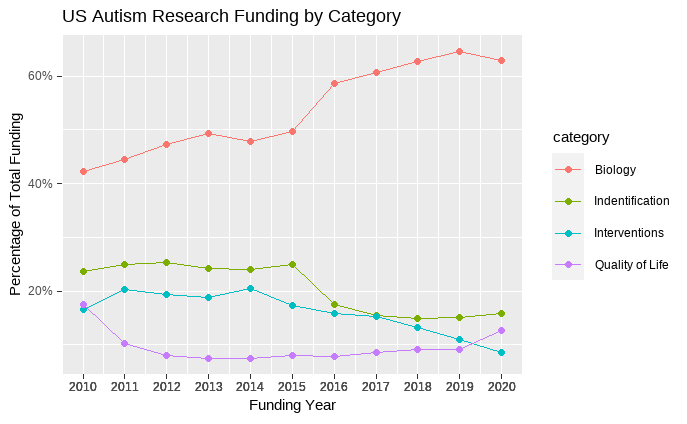
\includegraphics[width=5.4811in,height=\textheight]{././media/image1.png}

}

\caption{Figure 2. Data from {[}Interagency Autism Coordination
Committee{]}(https://iacc.hhs.gov/funding/data/)}

\end{figure}

\hypertarget{sec-marginalized}{%
\section{Intersectionally Marginalized Groups}\label{sec-marginalized}}

All of these problems compound for members of intersectional populations
who may already be marginalized along other dimensions. Many researchers
believe that autism is (Fombonne and Zuckerman 2022), particularly in
Black communities (Angell, Empey, and Zuckerman 2018), as well as for
(D'Mello et al. 2022). Meanwhile, fluidity in gender and sexual
orientation Rita George and Stokes (2018) is more highly represented
among autistic people. Little research has been done to assess how
autism uniquely affects people in these different subgroups.

\hypertarget{sec-physical_mental_health}{%
\section{Physical and Mental Health}\label{sec-physical_mental_health}}

\begin{itemize}
\tightlist
\item
  Health and Well-being: Autistic adults experience higher rates of
  mental health issues, physical health disparities, and substantially
  elevated suicide risk
  {[}\url{https://www.nature.com/articles/s41583-021-00463-7},
  \url{https://pubmed.ncbi.nlm.nih.gov/33407027/}{]}.
\item
  Social Isolation: Negative social experiences can lead to
  self-isolation, exacerbating feelings of loneliness and exclusion
  (Loomes, Hull, and Mandy 2017)
\end{itemize}

Across a variety of health domains, autistic people fare worse
Lodi-Smith, Rodgers, et al. (2021). Additionally, we are exposed to
risks that are not of primary concern for most people (Muskens, Velders,
and Staal 2017). These include autoimmune dysregulation of many kinds,
autonomic dysregulation, connective tissue disorders, gastrointestinal
disorders, and many other areas of health concerns. A lack of
understanding regarding these differences, coupled with communication
barriers and false notions about autism all collude to create barriers
to accessing health services and care.

\hypertarget{sec-unemployment}{%
\section{Unemployment}\label{sec-unemployment}}

\begin{itemize}
\tightlist
\item
  Employment: Many autistic adults face difficulties finding and
  maintaining employment due to biases and lack of accommodations. In a
  study of 254 autistic adults, 77\% reported difficulties applying for
  jobs, and only 16\% are in full-time paid work
  {[}\url{https://www.ncbi.nlm.nih.gov/pmc/articles/PMC5215190/},
  \url{https://www.frontiersin.org/articles/10.3389/fpsyg.2021.719827/full}{]}.
\end{itemize}

\hypertarget{sec-homelessness}{%
\section{Homelessness}\label{sec-homelessness}}

Barriers to entry to the workplace as well as challenges and holding
jobs due to ablest attitudes or inflexible policies put us at risk of
severe financial strain (Ohl et al. 2017). This coupled with the
possibility of reduced social support all increase our risk of exposure
to homelessness. The few studies that attempted to investigate autism in
homeless populations suggest that rates of autism in homeless
populations is much higher than that observed in the general public, and
may be ten times higher (Churchard et al. 2019). Autistic people
additionally face extra barriers in accessing the few services for
unhoused people. Environments created with the intention of providing
support may be aversive or even harmful for autistic people (Kargas et
al. 2019).

\hypertarget{sec-suicide}{%
\section{Suicide}\label{sec-suicide}}

As a group, their suicide risk may be two to seven times higher than the
risk for youth and adults who do not have autism. When researchers took
into account psychiatric conditions that increase suicide risk, such as
depression, anxiety, and substance abuse disorders, autistic people
still had a higher risk than the comparison group
{[}@\textbar autism2022{]}. The International Society for Autism
Research says ``Suicide in autism is a hidden crisis, overlooked by
policymakers, clinicians and researchers worldwide.'' and highlights
three barriers: a lack of evidence-based assessment tools and
interventions to identify and treat suicidal thoughts and behaviors; a
lack of access to mental health services10 and exclusion from
conversations about policies and guidelines that affect autistic
people.'' (Cassidy et al. 2021)

\hypertarget{appendix-glossary}{%
\chapter{Glossary}\label{appendix-glossary}}

\begin{longtable}[]{@{}
  >{\raggedright\arraybackslash}p{(\columnwidth - 2\tabcolsep) * \real{0.0376}}
  >{\raggedright\arraybackslash}p{(\columnwidth - 2\tabcolsep) * \real{0.9624}}@{}}
\toprule()
\begin{minipage}[b]{\linewidth}\raggedright
\textbf{Term}
\end{minipage} & \begin{minipage}[b]{\linewidth}\raggedright
\textbf{Definition}
\end{minipage} \\
\midrule()
\endhead
\textbf{ADLs} & When a person applies for Medicaid long-term care
services in Oregon, we look at how much help they need to perform
Activities of Daily Living. Because funding is limited, we use this
information (called a service priority level) to decide who is eligible
for services. Activities of Daily Living are the basic personal
activities all of us need to do that are essential for health and
safety. These activities are defined in OAR 411-015-0006
\href{https://www.oregon\%20.\%20gov/odhs/aging-disability-services/pages/adl.aspx}{\uline{https://www.oregon.gov/odhs/aging-disability-servi
ces/p ages/adl.aspx}} \\
\begin{minipage}[t]{\linewidth}\raggedright
\begin{itemize}
\tightlist
\item
  *A lexithymia**
\end{itemize}
\end{minipage} & Alexithymia is the inability for someone to recognize,
identify, and describe feelings or emotions. It is sometimes referred to
as emotional blindness.
\href{https://www.health.com/alexithymia-8361963}{{[}https://www.health.com/alexithymia-8361963{]}\{.unde
r line\}} \\
\textbf{Asperger's Syndrome} & Asperger's syndrome (sometimes called
high-functioning autism) is part of a wide diagnosis called autism
spectrum disorder (ASD). Since 2013, Asperger's syndrome is replaced by
the broader diagnosis of ASD within the Diagnostic and Statistical
Manual of Mental Disorders (DSM-5) revised criteria.
\href{https://my.clevelan\%20d\%20clinic.org/health/diseases/6436-asperger-syndrome}{\uline{h
t tps://my.clevelandclinic.org/health/diseases/6436- asper
ger-syndrome}} \\
\textbf{Co-Occurring Conditions} & The preferred term in the autistic
community as a replacement for ``comorbid'' for conditions, traits, and
behaviors that are commonly found along with autism. \\
\textbf{Double Empathy} & Double empathy refers to how:

1. It is easier to understand the mindset of people who are similar to
you

2. It is more difficult to understand the mindset of those who are
different from you

This concept was specifically developed by the autistic autism
researcher Damian Milton to explain how autistics and neurotypicals
empathize with each other. It explains how allistics (non-autistics)
struggle to understand the lived experiences of autistics and autistics
struggle to understand the lived experiences of allistics. Likewise,
autistics are better at understanding other autistics and allistics are
better at understanding other allistics.
\href{https://embrace\%20-\%20autism.com/autism-and-the-double-empathy-problem/}{\uline{https://embrace-autism.com/autism-and-the-do
uble- empathy-problem/}} \\
\textbf{Dyslexia} & Dyslexia is a specific learning difficulty which
primarily affects reading and writing skills. However, it does not only
affect these skills. Dyslexia is actually about information processing.
Dyslexic people may have difficulty processing and remembering
information they see and hear, which can affect learning and the
acquisition of literacy skills. Dyslexia can also impact on other areas
such as organisational skills. It is important to remember that there
are positives to thinking differently. Many dyslexic people show
strengths in areas such as reasoning and in visual and creative fields.
\href{https://www.bdadyslex\%20i\%20a.org.uk/dyslexia/about-dyslexia/what-is-dyslexia}{\uline{https
: //www.bdadyslexia.org.uk/dyslexia/about-dyslexia/w hat-i
s-dyslexia}} \\
\textbf{Dyspraxia} & Dyspraxia is a term that refers to lifelong trouble
with movement and coordination. It's not a formal diagnosis. But you may
still hear people use this term, especially in the U.K. The formal
diagnosis is developmental coordination disorder (DCD).
\href{https://www.\%20u\%20nderstood.org/en/articles/understanding-dyspraxia}{\uline{https://www.understood.org/en/articles
/unde rstanding-dyspraxia}} \\
\textbf{fMRI} & Functional MRI is a type of MRI scan that can show which
areas of your brain are most active. Tracking and comparing that
activity to what you were doing at the time can help ``map'' your brain
activity. It's most often used for planning surgery or similar
procedures in the brain.
\href{https://my.clevelandclini\%20c\%20.org/health/diagnostics/25034-functional-mri-fmri}{\uline{https://my.cl
e velandclinic.org/health/diagnostics/25034-function al-mr i-fmri}} \\
\textbf{Gender identity} & One's innermost concept of self as male,
female, a blend of both or neither -- how individuals perceive
themselves and what they call themselves. One's gender identity can be
the same or different from their sex assigned at birth.
\href{https://www.hrc.org/resources/sexual-orientati\%20o\%20n-and-gender-identity-terminology-and-definitions}{{[}http
s ://www.hrc.org/resources/sexual-orientation-and-ge n
der-identity-terminology-and-definitions{]}\{.underli ne\}} \\
\textbf{Genome} & The genome is the entire set of DNA instructions found
in a cell. In humans, the genome consists of 23 pairs of chromosomes
located in the cell's nucleus, as well as a small chromosome in the
cell's mitochondria. A genome contains all the information needed for an
individual to develop and function.
\href{https://www.genome.gov/genetics-glossary/Genome}{\uline{https://
ww w.genome.gov/genetics-glossary/Genome}} \\
\textbf{Health Share Oregon} & One of Oregon's Community Care
Organizations (CCO) for OHP.
\href{https://www.healthshareoregon.org/}{\uline{https://www.healthshareoregon.org
/}} \\
\textbf{I/DD} &
\href{h\%20ttps://www.oregon.gov/odhs/idd/pages/default.aspx}{\uline{Oregon
Department of Human Services: Intellectual and Developmental
Disabilities.}} \\
\textbf{Letter of Medical Necessity} & A Letter of Medical Necessity
(LMN) is the written explanation from the treating physician describing
the medical need for services, equipment, or supplies to assist the
claimant in the treatment, care, or relief of their accepted
work-related illness(es). \url{https://www.dol} .
gov/sites/dolgov/files/OWCP/energy/regs/compliance /
Outreach/Outreach\_Presentation/lmn\_mba06222022.pdf \\
\textbf{Ne urodivergent} & \\
\textbf{Ne urodiversity} & \\
\textbf{Non-Speaking} & When an autistic person doesn't speak, it's
known as nonspeaking autism. You may also see it described as nonverbal
autism. However, the term nonverbal isn't completely accurate, since it
means ``without words. Even if an autistic person is nonspeaking, they
may still use words in other ways (such as in writing). They may also
understand the words that are spoken to them or that they overhear.
https: / /www.healthline.com/health/autism/nonverbal-autism \\
\textbf{OCD} & Obsessive-compulsive disorder (OCD) is a disorder in
which people have recurring, unwanted thoughts, ideas or sensations
(obsessions). To get rid of the thoughts, they feel driven to do
something repetitively (compulsions). The repetitive behaviors, such as
hand washing/cleaning, checking on things, and mental acts like
(counting) or other activities, can significantly interfere with a
person's daily activities and social interactions. \url{https://ww} w
.psychiatry.org/patients-families/obsessive-compul s
ive-disorder/what-is-obsessive-compulsive-disorder \\
\textbf{ODDS} & Oregon
\href{https://ww\%20w\%20.oregon.gov/odhs/agency/pages/odds.aspx?jump=true}{\uline{Office
of Developmental Disabilities Services}} \\
\textbf{OHP} &
\href{h\%20t\%20tps://www.oregon.gov/oha/hsd/ohp/pages/index.aspx}{\uline{Oregon
Health Plan: Oregon Medicaid}} \\
\textbf{Services Cliff} & Many high school students on the autism
spectrum get help through special education -- most commonly including
speech-language therapy, service coordination/case management, behavior
management, and special transportation. Each student has a team that
works with the student and family to decide which services are needed to
prepare him or her for young adulthood, and federal law requires schools
to offer the necessary services. Sounds like a good plan for how to help
vulnerable youth through a challenging period of life. But then,
following the last day of high school, the legal mandate for help
suddenly ends.
\href{https://drexel.edu/autismoutcomes/blog/ov\%20e\%20rview/2015/August/falling-off-the-services-cliff/}{{[}https://drexel.edu/autismoutcomes/blog/overvi
e w/2015/August/falling-off-the-services-cliff/{]}\{.un derli ne\}} \\
\textbf{Sexual orientation} & An inherent or immutable enduring
emotional, romantic or sexual attraction to other people. Note: an
individual's sexual orientation is independent of their gender identity.
\href{https://www.hrc.org/resources/sexual-orientati\%20o\%20n-and-gender-identity-terminology-and-definitions}{{[}http
s ://www.hrc.org/resources/sexual-orientation-and-ge n
der-identity-terminology-and-definitions{]}\{.underli ne\}} \\
\begin{minipage}[t]{\linewidth}\raggedright
\begin{itemize}
\tightlist
\item
  *S ynesthesia**
\end{itemize}
\end{minipage} & Synesthesia is when your brain routes sensory
information through multiple unrelated senses, causing you to experience
more than one sense simultaneously. Some examples include tasting words
or linking colors to numbers and letters. It's not a medical condition,
and many people find it useful to help them learn and remember
information. \url{https://my.cl} e
velandclinic.org/health/symptoms/24995-synesthesia \\
\textbf{Theory of Mind} & In psychology, theory of mind refers to the
capacity to understand other people by ascribing mental states to them.
A theory of mind includes the knowledge that others' beliefs, desires,
intentions, emotions, and thoughts may be different from one's own.
Possessing a functional theory of mind is crucial for success in
everyday human social interactions. People utilize a theory of mind when
analyzing, judging, and inferring others' behaviors. The discovery and
development of theory of mind primarily came from studies done with
animals and infants. Factors including drug and alcohol consumption,
language development, cognitive delays, age, and culture can affect a
person's capacity to display theory of mind. Having a theory of mind is
similar to but not identical with having the capacity for empathy or
sympathy. \url{https://en.wikipedia.org/wiki/Theory_of_mind} \\
\bottomrule()
\end{longtable}

\hypertarget{section-6}{%
\chapter{}\label{section-6}}

\hypertarget{appendix-representative-salaries}{%
\chapter{Representative
Salaries}\label{appendix-representative-salaries}}

\begin{longtable}[]{@{}
  >{\raggedright\arraybackslash}p{(\columnwidth - 8\tabcolsep) * \real{0.2941}}
  >{\raggedright\arraybackslash}p{(\columnwidth - 8\tabcolsep) * \real{0.1882}}
  >{\raggedright\arraybackslash}p{(\columnwidth - 8\tabcolsep) * \real{0.1647}}
  >{\raggedright\arraybackslash}p{(\columnwidth - 8\tabcolsep) * \real{0.1529}}
  >{\raggedright\arraybackslash}p{(\columnwidth - 8\tabcolsep) * \real{0.1647}}@{}}
\toprule()
\begin{minipage}[b]{\linewidth}\raggedright
Data Analyst
\end{minipage} & \begin{minipage}[b]{\linewidth}\raggedright
\end{minipage} & \begin{minipage}[b]{\linewidth}\raggedright
\end{minipage} & \begin{minipage}[b]{\linewidth}\raggedright
\end{minipage} & \begin{minipage}[b]{\linewidth}\raggedright
\end{minipage} \\
\midrule()
\endhead
& Annual Salary & Monthly Pay & Weekly Pay & Hourly Wage \\
Top Earners & \$ 127,790.00 &
\begin{minipage}[t]{\linewidth}\raggedright
\hfill\break
\$10,649.00\strut
\end{minipage} & \$2,458.00 & \$61.00 \\
75th Percentile & \$ 102,900.00 & \$8,575.00 & \$1,979.00 & \$49.00 \\
Average & \begin{minipage}[t]{\linewidth}\raggedright
\hfill\break
\$87,640.00\strut
\end{minipage} & \$7,303.00 & \$1,685.00 & \$42.00 \\
25th Percentile & \begin{minipage}[t]{\linewidth}\raggedright
\hfill\break
\$66,300.00\strut
\end{minipage} & \$5,525.00 & \$1,275.00 & \$32.00 \\
Data Engineer & & & & \\
& Annual Salary & Monthly Pay & Weekly Pay & Hourly Wage \\
Top Earners & \$ 171,801.00 &
\begin{minipage}[t]{\linewidth}\raggedright
\hfill\break
\$14,316.00\strut
\end{minipage} & \$3,303.00 & \$83.00 \\
75th Percentile & \$ 145,800.00 &
\begin{minipage}[t]{\linewidth}\raggedright
\hfill\break
\$12,150.00\strut
\end{minipage} & \$2,803.00 & \$70.00 \\
Average & \$ 138,279.00 & \begin{minipage}[t]{\linewidth}\raggedright
\hfill\break
\$11,523.00\strut
\end{minipage} & \$2,659.00 & \$66.00 \\
25th Percentile & \$ 121,400.00 &
\begin{minipage}[t]{\linewidth}\raggedright
\hfill\break
\$10,116.00\strut
\end{minipage} & \$2,334.00 & \$58.00 \\
Database Administrator & & & & \\
& Annual Salary & Monthly Pay & Weekly Pay & Hourly Wage \\
Top Earners & \$ 150,061.00 &
\begin{minipage}[t]{\linewidth}\raggedright
\hfill\break
\$12,505.00\strut
\end{minipage} & \$2,886.00 & \$72.00 \\
75th Percentile & \$ 130,400.00 &
\begin{minipage}[t]{\linewidth}\raggedright
\hfill\break
\$10,867.00\strut
\end{minipage} & \$2,508.00 & \$63.00 \\
Average & \$ 108,448.00 & \$9,037.00 & \$2,086.00 & \$52.00 \\
25th Percentile & \begin{minipage}[t]{\linewidth}\raggedright
\hfill\break
\$84,800.00\strut
\end{minipage} & \$7,067.00 & \$1,631.00 & \$41.00 \\
Director of Operations & & & & \\
& Annual Salary & Monthly Pay & Weekly Pay & Hourly Wage \\
Top Earners & \$ 171,801.00 &
\begin{minipage}[t]{\linewidth}\raggedright
\hfill\break
\$14,316.00\strut
\end{minipage} & \$3,303.00 & \$83.00 \\
75th Percentile & \$ 143,700.00 &
\begin{minipage}[t]{\linewidth}\raggedright
\hfill\break
\$11,975.00\strut
\end{minipage} & \$2,763.00 & \$69.00 \\
Average & \$ 102,922.00 & \$8,576.00 & \$1,979.00 & \$49.00 \\
25th Percentile & \begin{minipage}[t]{\linewidth}\raggedright
\hfill\break
\$80,100.00\strut
\end{minipage} & \$6,675.00 & \$1,540.00 & \$39.00 \\
Grant Writer & & & & \\
& Annual Salary & Monthly Pay & Weekly Pay & Hourly Wage \\
Top Earners & \begin{minipage}[t]{\linewidth}\raggedright
\hfill\break
\$91,733.00\strut
\end{minipage} & \$7,644.00 & \$1,764.00 & \$44.00 \\
75th Percentile & \begin{minipage}[t]{\linewidth}\raggedright
\hfill\break
\$77,900.00\strut
\end{minipage} & \$6,492.00 & \$1,498.00 & \$37.00 \\
Average & \begin{minipage}[t]{\linewidth}\raggedright
\hfill\break
\$70,107.00\strut
\end{minipage} & \$5,842.00 & \$1,348.00 & \$34.00 \\
25th Percentile & \begin{minipage}[t]{\linewidth}\raggedright
\hfill\break
\$55,100.00\strut
\end{minipage} & \$4,592.00 & \$1,060.00 & \$26.00 \\
Director of Operations & & & & \\
& Annual Salary & Monthly Pay & Weekly Pay & Hourly Wage \\
Top Earners & \$ 171,801.00 &
\begin{minipage}[t]{\linewidth}\raggedright
\hfill\break
\$14,316.00\strut
\end{minipage} & \$3,303.00 & \$83.00 \\
75th Percentile & \$ 143,700.00 &
\begin{minipage}[t]{\linewidth}\raggedright
\hfill\break
\$11,975.00\strut
\end{minipage} & \$2,763.00 & \$69.00 \\
Average & \$ 102,922.00 & \$8,576.00 & \$1,979.00 & \$49.00 \\
25th Percentile & \begin{minipage}[t]{\linewidth}\raggedright
\hfill\break
\$80,100.00\strut
\end{minipage} & \$6,675.00 & \$1,540.00 & \$39.00 \\
Operations Manager & & & & \\
& Annual Salary & Monthly Pay & Weekly Pay & Hourly Wage \\
Top Earners & \$ 115,064.00 & \$9,588.00 & \$2,212.00 & \$55.00 \\
75th Percentile & \begin{minipage}[t]{\linewidth}\raggedright
\hfill\break
\$82,200.00\strut
\end{minipage} & \$6,850.00 & \$1,580.00 & \$40.00 \\
Average & \begin{minipage}[t]{\linewidth}\raggedright
\hfill\break
\$68,498.00\strut
\end{minipage} & \$5,708.00 & \$1,317.00 & \$33.00 \\
25th Percentile & \begin{minipage}[t]{\linewidth}\raggedright
\hfill\break
\$43,500.00\strut
\end{minipage} & \$3,625.00 & \$836.00 & \$21.00 \\
Policy Analyst & & & & \\
& Annual Salary & Monthly Pay & Weekly Pay & Hourly Wage \\
Top Earners & \$ 123,548.00 &
\begin{minipage}[t]{\linewidth}\raggedright
\hfill\break
\$10,295.00\strut
\end{minipage} & \$2,375.00 & \$59.00 \\
75th Percentile & \$ 123,500.00 &
\begin{minipage}[t]{\linewidth}\raggedright
\hfill\break
\$10,291.00\strut
\end{minipage} & \$2,375.00 & \$59.00 \\
Average & \begin{minipage}[t]{\linewidth}\raggedright
\hfill\break
\$97,464.00\strut
\end{minipage} & \$8,122.00 & \$1,874.00 & \$47.00 \\
25th Percentile & \begin{minipage}[t]{\linewidth}\raggedright
\hfill\break
\$88,000.00\strut
\end{minipage} & \$7,333.00 & \$1,692.00 & \$42.00 \\
Research Associate & & & & \\
& Annual Salary & Monthly Pay & Weekly Pay & Hourly Wage \\
Top Earners & \begin{minipage}[t]{\linewidth}\raggedright
\hfill\break
\$94,915.00\strut
\end{minipage} & \$7,910.00 & \$1,825.00 & \$46.00 \\
75th Percentile & \begin{minipage}[t]{\linewidth}\raggedright
\hfill\break
\$81,700.00\strut
\end{minipage} & \$6,808.00 & \$1,571.00 & \$39.00 \\
Average & \begin{minipage}[t]{\linewidth}\raggedright
\hfill\break
\$71,781.00\strut
\end{minipage} & \$5,982.00 & \$1,380.00 & \$35.00 \\
25th Percentile & \begin{minipage}[t]{\linewidth}\raggedright
\hfill\break
\$57,800.00\strut
\end{minipage} & \$4,817.00 & \$1,112.00 & \$28.00 \\
Senior Manager & & & & \\
& Annual Salary & Monthly Pay & Weekly Pay & Hourly Wage \\
Top Earners & \$ 178,695.00 &
\begin{minipage}[t]{\linewidth}\raggedright
\hfill\break
\$14,891.00\strut
\end{minipage} & \$3,436.00 & \$86.00 \\
75th Percentile & \$ 144,800.00 &
\begin{minipage}[t]{\linewidth}\raggedright
\hfill\break
\$12,066.00\strut
\end{minipage} & \$2,784.00 & \$70.00 \\
Average & \begin{minipage}[t]{\linewidth}\raggedright
\hfill\break
\$93,748.00\strut
\end{minipage} & \$7,812.00 & \$1,802.00 & \$45.00 \\
25th Percentile & \begin{minipage}[t]{\linewidth}\raggedright
\hfill\break
\$52,000.00\strut
\end{minipage} & \$4,333.00 & \$1,000.00 & \$25.00 \\
Website Designer & & & & \\
& Annual Salary & Monthly Pay & Weekly Pay & Hourly Wage \\
Top Earners & \$ 109,232.00 & \$9,103.00 & \$2,101.00 & \$53.00 \\
75th Percentile & \begin{minipage}[t]{\linewidth}\raggedright
\hfill\break
\$84,800.00\strut
\end{minipage} & \$7,067.00 & \$1,631.00 & \$41.00 \\
Average & \begin{minipage}[t]{\linewidth}\raggedright
\hfill\break
\$77,227.00\strut
\end{minipage} & \$6,436.00 & \$1,485.00 & \$37.00 \\
25th Percentile & \begin{minipage}[t]{\linewidth}\raggedright
\hfill\break
\$56,700.00\strut
\end{minipage} & \$4,725.00 & \$1,090.00 & \$27.00 \\
Website Programmer & & & & \\
& Annual Salary & Monthly Pay & Weekly Pay & Hourly Wage \\
Top Earners & \$ 119,306.00 & \$9,942.00 & \$2,294.00 & \$57.00 \\
75th Percentile & \$ 100,700.00 & \$8,392.00 & \$1,937.00 & \$48.00 \\
Average & \begin{minipage}[t]{\linewidth}\raggedright
\hfill\break
\$85,087.00\strut
\end{minipage} & \$7,091.00 & \$1,636.00 & \$41.00 \\
25th Percentile & \begin{minipage}[t]{\linewidth}\raggedright
\hfill\break
\$67,300.00\strut
\end{minipage} & \$5,608.00 & \$1,294.00 & \$32.00 \\
\bottomrule()
\end{longtable}

\hypertarget{section-7}{%
\chapter{}\label{section-7}}

\hypertarget{appendix-potential-funders}{%
\chapter{Potential Funders}\label{appendix-potential-funders}}

\hypertarget{healthcare-corporations}{%
\section{Healthcare Corporations}\label{healthcare-corporations}}

\begin{longtable}[]{@{}
  >{\raggedright\arraybackslash}p{(\columnwidth - 4\tabcolsep) * \real{0.1644}}
  >{\raggedright\arraybackslash}p{(\columnwidth - 4\tabcolsep) * \real{0.1644}}
  >{\raggedright\arraybackslash}p{(\columnwidth - 4\tabcolsep) * \real{0.6712}}@{}}
\toprule()
\begin{minipage}[b]{\linewidth}\raggedright
Or ganiz ation
\end{minipage} & \begin{minipage}[b]{\linewidth}\raggedright
Pr oduct
\end{minipage} & \begin{minipage}[b]{\linewidth}\raggedright
Links
\end{minipage} \\
\midrule()
\endhead
Adve ntist & S ponso rship Re quest &
\href{https://hipaa-submit.jotform.com/221594871753061}{\uline{https://hi
paa-submit.jotform.com/221594871753061}} \\
Adve ntist & Comm unity Be nefit &
\href{https://advent\%20isthealth.org/portland/about-us/community-benefit/}{\uline{https://adventisthealth.org/portland/about
-us/community-benefit/}} \\
C ambia & He althy and Conn ected Aging &
\href{https://www.cambiahealthfoundatio\%20n.org/focus-areas/healthy-and-connected-aging.html}{\uline{https://www.cambiahealthfound
ation.org/focus-areas/healthy-and-connected-aging.h tml}} \\
C ambia & S ponso rship &
\href{https://www.cambiahealthfoundation.org/appl\%20icant-resources/current-funding-opportunities.html}{{[}https://www.cambiahealthfoundation.org/applicant-
resources/current-funding-opportunities.html{]}\{.unde rline\}} \\
CareO regon & Comm unity G iving g rants and sp onsor ships &
\href{https://www.careoregon.org/community/c\%20ommunity-giving-grants-for-nonprofit-organizations}{\uline{https://www.careoregon.org/community/co
mmunity-giving-grants-for-nonprofit-organizations}} \\
CareO regon & HRSN Ser vices &
\href{mailto:r\%20equest.social.determinants@careoregon.org}{re
quest.social.determinants@careoregon.org}, \\
H ealth Share & S ponso rship &
\href{h\%20ttps://www.healthshareoregon.org/about/sponsorship}{\uline{https://www.heal
thshareoregon.org/about/sponsorship}} \\
H ealth Share & HRSN Ser vices &
\href{https:/\%20/www.healthshareoregon.org/community-partners/hrsn}{\uline{https://www.healthshareorego
n.org/community-partners/hrsn}} \\
H ealth Share & HRSN Ser vices &
\href{https://health-share-or.portals.zeng\%20inehq.com/program/community-capacity-building/info}{\uline{https://health-share-or.portals.zen
ginehq.com/program/community-capacity-building/info}} \\
K aiser & HRSN Ser vices &
\href{mailto:Laura.J.Howard@kp.org}{Laura.J.Ho ward@kp.org} \\
K aiser & HRSN Ser vices &
\href{https://communityhealth-midatlantic.kaise\%20rpermanente.org/improving-communities/grantmaking/}{{[}https://communityhealth-midatlantic.kaiserper
manente.org/improving-communities/grantmaking/{]}\{.un derline\}} \\
K aiser & HRSN Ser vices &
\href{https://communityh\%20ealth-midatlantic.kaiserpermanente.org/wp-content/u\%20ploads/2024/02/LOI-Submitter-Help-Document_508.pdf}{\uline{https://communityhealth-midatlantic.kaiserpermanen
te.org/wp-content/uploads/2024/02/LOI-Submitter-Hel
p-Document\_508.pdf}} \\
K aiser & HRSN Ser vices &
\href{mailto:MedicaidHRSflexfunds@kp.org}{MedicaidHRSflexfunds@
kp.org} \\
K aiser & Comm unity Be nefit &
\href{mailto:community.benefit@kp.org}{community.benefi t@kp.org} \\
L egacy & Comm unity H ealth Grant &
\href{https://www.legacyhealth.org/Giving\%20-and-Support/community-engagement/Community-Grants}{\uline{https://www.legacyhealth.org/Givi
ng-and-Support/community-engagement/Community-Grant s}} \\
L egacy & L egacy Res earch Inst itute &
\href{https://www.legacyhealth.org/For-Health-Profe\%20ssionals/legacy-research-institute/services/grants}{{[}ht
tps://www.legacyhealth.org/For-Health-Professionals
/legacy-research-institute/services/grants{]}\{.underl ine\}} \\
L egacy & S ponso rship &
\href{https://www.legacyhealth.org/Gi\%20ving-and-Support/community-engagement/Sponsorships}{\uline{https://www.legacyhealth.
org/Giving-and-Support/community-engagement/Sponsor ships}} \\
L egacy & HRSN Ser vices &
\href{mail\%20to:HealthRelatedServices@pacificsource.com}{HealthRelatedServices@pacificsource.com} \\
Ochin & & \\
OHSU & Comm unity P artne rship Pr ogram &
\href{https://www.ohsu.edu/knight-can\%20cer-institute/community-partnership-program-grants}{\uline{https://www.ohsu.edu/knig
ht-cancer-institute/community-partnership-program-g rants}} \\
OHSU & Comm unity P artne rship Pr ogram &
\href{https://www.ohsu.edu\%20/knight-cancer-institute/how-apply-community-grant}{\uline{htt
ps://www.ohsu.edu/knight-cancer-institute/how-apply
-community-grant}} \\
OHSU & Comm unity P artne rship Pr ogram &
\href{https://www.ohsu.edu/sites/defau\%20lt/files/2024-01/CPP_RFP_2024.1_FINAL_lowres_0.pdf}{\uline{https://www.ohsu.edu/sites/
default/files/2024-01/CPP\_RFP\_2024.1\_FINAL\_lowres\_0 .pdf}} \\
OHSU & T iered G rants &
\href{https://\%20www.ohsu.edu/knight-cancer-institute/tiered-grants}{\uline{https://www.ohsu.edu/knight-ca
ncer-institute/tiered-grants}} \\
OHSU & HRSN Ser vices &
\href{https://www.ohsu.edu/health-services}{{[}https://www.ohsu.edu/health-services{]}
\{.underline\}} \\
OHSU & Rural Popul ation H ealth Incu bator Pr ogram &
\href{https://www.ohsu.edu/oregon-office-of-rura\%20l-health/rural-population-health-incubator-program}{{[}https://www.ohsu.edu/oregon-office-of-rural-hea
lth/rural-population-health-incubator-program{]}\{.und erline\}} \\
Pa cific S ource & Comm unity H ealth Excel lence G rants &
\href{https://pacificsource.com/sites\%20/default/files/2023-02/PRV510_0123_CHE\%20Flier.pdf}{\uline{https://pacificsource.com
/sites/default/files/2023-02/PRV510\_0123\_CHE\%20Flie r.pdf}} \\
Pa cific S ource & Comm unity Ca pacit y-Bui lding Fu nding for HRSN ser
vices &
\href{https://pacificsource.com/article\%20/community-capacity-building-funding-hrsn-services}{\uline{https://pacificsource.com/art
icle/community-capacity-building-funding-hrsn-servi ces}} \\
Pa cific S ource & Comm unity H ealth Excel lence G rants &
\href{https://www.ruralhealthinfo.org/funding/5469}{{[}ht
tps://www.ruralhealthinfo.org/funding/5469{]}\{.underl ine\}} \\
Pa cific S ource & All &
\href{https://pacifi\%20csource.com/sites/default/files/2023-08/CLB1330_082\%203_PacificSource\%20Funding\%20Navigation\%20Guide.pdf}{\uline{https://pacificsource.com/sites/default/fi
les/2023-08/CLB1330\_0823\_PacificSource\%20Funding\%20
Navigation\%20Guide.pdf}} \\
Pa cific S ource & Pac ificS ource Found ation for H ealth I mprov ement
&
\href{https://pacificsou\%20rce.com/community/foundation?utm_source=pdf\&utm_med\%20ium=flier\&utm_campaign=FundingGuide\&utm_id=CLB1330}{\uline{https://pacificsource.com/community/foundation?utm
\_source=pdf\&utm\_medium=flier\&utm\_campaign=FundingGu
ide\&utm\_id=CLB1330}} \\
Pa cific S ource & He althy C ommun ities Pr ogram &
\href{http://www.grantinterface.com/Home/Logon}{{[}http://www.grantinterface.com/Home/Logon{]}\{.un
derline\}} \\
Provi dence & Comm unity G rants /Dona tions &
\href{https://www.providence.or\%20g/locations/wa/providence-regional-medical-center-e\%20verett/donate-and-volunteer/community-sponsorships}{\uline{https://www.p
rovidence.org/locations/wa/providence-regional-medi
cal-center-everett/donate-and-volunteer/community-s ponsorships}} \\
Provi dence & S ponso rship &
\href{https://w\%20ebportalapp.com/sp/login/prmce-sponsor-application}{\uline{https://webportalapp.com/sp/logi
n/prmce-sponsor-application}} \\
Provi dence & HRSN Ser vices &
\href{mailto:HRSNBenefit@Providence.org}{HRSNBenefit@Provide nce.org} \\
Tri llium & Comm unity Be nefit I nitia tives &
\href{https://www.prnewswire.co\%20m/news-releases/trillium-community-health-plan-anno\%20unces-request-for-applications-for-2023-small-grant\%20s-for-community-benefit-initiatives-301845411.html}{\uline{https://www.p
rnewswire.com/news-releases/trillium-community-heal
th-plan-announces-request-for-applications-for-2023
-small-grants-for-community-benefit-initiatives-301 845411.html}} \\
Tri llium & Comm unity Be nefit I nitia tives &
\href{https://www.trilliumohp.com/supporting-ore\%20gon-communities/community-benefit-initiatives.html}{{[}https://www.trilliumohp.com/supporting-oregon-c
ommunities/community-benefit-initiatives.html{]}\{.und erline\}} \\
Tri llium & Comm unity Cap acity Bui lding Fu nding &
\href{https://www.trilliumohp.c\%20om/supporting-oregon-communities/health-related-soc\%20ial-needs/community-capacity-building-funding.html}{\uline{https://www.t
rilliumohp.com/supporting-oregon-communities/health
-related-social-needs/community-capacity-building-f unding.html}} \\
Ce ntral O regon H ealth Co uncil & Sta ndard G rants &
\href{https://cohealthcouncil.org/standard-grants/}{{[}ht
tps://cohealthcouncil.org/standard-grants/{]}\{.underl ine\}} \\
& Mini G rants &
\href{https://cohealthcouncil.org/mini-grants/}{{[}https://cohealthcouncil.org/mini-grants/{]}\{.un
derline\}} \\
St Ch arles H ealth S ystem & Comm unity Be nefit G rants and Sp onsor
ships &
\href{https://www.stcharleshealthcare.org/communit\%20y-health/community-benefit-grants-and-sponsorships}{{[}
https://www.stcharleshealthcare.org/community-healt
h/community-benefit-grants-and-sponsorships{]}\{.under line\}} \\
\bottomrule()
\end{longtable}

\hypertarget{state-agencies}{%
\section{State Agencies}\label{state-agencies}}

\begin{longtable}[]{@{}
  >{\raggedright\arraybackslash}p{(\columnwidth - 4\tabcolsep) * \real{0.1528}}
  >{\raggedright\arraybackslash}p{(\columnwidth - 4\tabcolsep) * \real{0.1528}}
  >{\raggedright\arraybackslash}p{(\columnwidth - 4\tabcolsep) * \real{0.6944}}@{}}
\toprule()
\begin{minipage}[b]{\linewidth}\raggedright
Entity
\end{minipage} & \begin{minipage}[b]{\linewidth}\raggedright
P roduct
\end{minipage} & \begin{minipage}[b]{\linewidth}\raggedright
Links
\end{minipage} \\
\midrule()
\endhead
Oregon Health Aut hority & Block Grants &
\href{https://www.or\%20egon.gov/oha/hsd/amhpac/pages/block-grants.aspx}{\uline{https://www.oregon.gov/oha/hsd/amhpac/page
s/block-grants.aspx}} \\
Oregon Health Aut hority & Com munity Ca pacity Bu ilding Funds &
\href{https://www.ore\%20gon.gov/oha/hsd/medicaid-policy/pages/ccbf.aspx}{\uline{https://www.oregon.gov/oha/hsd/medicaid-poli
cy/pages/ccbf.aspx}} \\
Oregon Health Aut hority & Com munity Ca pacity Bu ilding Funds &
\href{https://content.\%20govdelivery.com/accounts/ORHA/bulletins/38e15e8}{\uline{https://content.govdelivery.com/accounts/ORHA/
bulletins/38e15e8}} \\
Oregon Health Aut hority & SHARE Init iative &
\href{https:/\%20/www.oregon.gov/oha/hpa/dsi-tc/pages/share.aspx}{\uline{https://www.oregon.gov/oha/h
pa/dsi-tc/pages/share.aspx}} \\
Oregon Health Aut hority & PUBLIC HEALTH EQUITY &
\url{https://www.oregon.gov/oha/PH/ABOUT/MODCE}
T\%20CBO\%20Documents/PH\%20Equity\%20CBO\%20Fiscal\%2
0Guidance\%20-\%20AY25\%20\%20DRAFT-\%2002.28.24.pdf\textgreater{} \\
Oregon Health Aut hority & PUBLIC HEALTH EQUITY &
\href{https://content.\%20govdelivery.com/accounts/ORHA/bulletins/37611cc}{\uline{https://content.govdelivery.com/accounts/ORHA/
bulletins/37611cc}} \\
Oregon Health Aut hority & GRANT &
\href{https://www.oregon.gov/oha/ph/\%20healthypeoplefamilies/youth/healthschool/schoolb\%20asedhealthcenters/pages/mh-expansion-grant.aspx}{\uline{https://www.oregon.gov/oha
/ph/healthypeoplefamilies/youth/healthschool/sch
oolbasedhealthcenters/pages/mh-expansion-grant.a spx}} \\
Oregon Health Aut hority & HTO CHIP P roject Grants &
\href{https://www.oregon.gov/oha\%20/PH/ABOUT/Documents/HTO\%20CHIP\%202024\%20FAQ.pdf}{\uline{https://www.oregon
.gov/oha/PH/ABOUT/Documents/HTO\%20CHIP\%202024\%20 FAQ.pdf}} \\
Oregon State & I MPACTS Grant P rogram &
\href{https://www.oregon.gov\%20/cjc/impacts/Documents/2020_IMPACTSOnePager.pdf}{\uline{https://ww
w.oregon.gov/cjc/impacts/Documents/2020\_IMPACTSO nePager.pdf}} \\
\bottomrule()
\end{longtable}

\hypertarget{foundations-and-trusts}{%
\section{Foundations and Trusts}\label{foundations-and-trusts}}

\begin{longtable}[]{@{}
  >{\raggedright\arraybackslash}p{(\columnwidth - 4\tabcolsep) * \real{0.1806}}
  >{\raggedright\arraybackslash}p{(\columnwidth - 4\tabcolsep) * \real{0.1806}}
  >{\raggedright\arraybackslash}p{(\columnwidth - 4\tabcolsep) * \real{0.6389}}@{}}
\toprule()
\begin{minipage}[b]{\linewidth}\raggedright
Foun dation
\end{minipage} & \begin{minipage}[b]{\linewidth}\raggedright
P roduct
\end{minipage} & \begin{minipage}[b]{\linewidth}\raggedright
Links
\end{minipage} \\
\midrule()
\endhead
Car penter Foun dation & Grant &
\href{http://carpenter-foundation.org/}{\uline{http://carpenter-foundation.or
g/}} \\
Anna May Family Foun dation & Grant &
\href{http://www.annamay.org/}{\uline{http://www.a nnamay.org/}} \\
Gordon Elwood Foun dation & Grant &
\href{https://www.gordonelwoodfoundation.org/index}{{[}http
s://www.gordonelwoodfoundation.org/index{]}\{.underli ne\}} \\
Ma ybelle Clark Mac donald Fund & Grant &
\href{https://mcmfundgiving.org/grants/}{\uline{https://mcmfundgiving.org/grants
/}} \\
M J M urdock Char itable Trust & STR ATEGIC GRANT &
\href{ht\%20tps://murdocktrust.org/grant-application-process/}{\uline{https://murdocktru
st.org/grant-application-process/}} \\
C ollins Foun dation & Resp onsive Grant &
\href{https://www.collinsfoundation\%20.org/responsive-grantmaking-submission-guidelines}{\uline{https://www.collinsfou
ndation.org/responsive-grantmaking-submission-guid elines}} \\
C ollins Foun dation & Resp onsive Grant &
\href{https:\%20//www.collinsfoundation.org/responsive-grantmaking\%20-submission-guidelines/frequently-asked-questions}{\uline{https://www.collinsfoundat
ion.org/responsive-grantmaking-submission-guidelin
es/frequently-asked-questions}} \\
Benton Com munity Foun dation & Com munity Grants &
\href{https://bcfgives.org/wp-co\%20ntent/uploads/2024/02/2023-Full-Grant-History.pdf}{\uline{https://bcfgives
.org/wp-content/uploads/2024/02/2023-Full-Grant-Hi story.pdf}} \\
Reser Family Foun dation & Resp onsive Grant Pr ograms &
\href{https:\%20//thereserfamilyfoundation.org/apply-for-a-grant/}{\uline{https://thereserfamilyfoun
dation.org/apply-for-a-grant/}} \\
Foster Foun dation & Grant &
\href{http://www.thefosterfoundation.org/Home.htm}{{[}ht
tp://www.thefosterfoundation.org/Home.htm{]}\{.underl ine\}} \\
Doug Flutie Foun dation & Autism Com munity Impact Grant &
\href{https://flutiefoundation.org/h\%20elping-communities/autism-community-impact-grant/}{\uline{https://flutiefoundation
.org/helping-communities/autism-community-impact-g rant/}} \\
Doug Flutie Foun dation & Flutie F ellows -- Career and Life Goal S
upport &
\href{https://flutiefoundation.org/helping-individ\%20uals/flutie-fellows-career-and-life-goal-support/}{{[}ht
tps://flutiefoundation.org/helping-individuals/flu
tie-fellows-career-and-life-goal-support/{]}\{.underl ine\}} \\
Doug Flutie Foun dation & Fin ancial Relief for Fa milies &
\href{https://flutiefoundati\%20on.org/helping-families/direct-financial-support/}{\uline{https://
flutiefoundation.org/helping-families/direct-finan cial-support/}} \\
Ch ambers Family Foun dation & Grant &
\href{htt\%20ps://www.chambersfamilyfoundation.com/submissions}{\uline{https://www.chambers
familyfoundation.com/submissions}} \\
Meyer Me morial Trust & Grant &
\href{https://mmt.org/}{\uline{https://mmt.org/}} \\
Ben B Cheney Foun dation & Grant &
\href{https://www.benbcheneyfoundation.org/}{{[}https://www.benbcheneyfoundation.org/{]}\{.
underline\}} \\
Autzen Foun dation & Grant &
\href{https://www.autzenfoundation.org/deadlines}{{[}
https://www.autzenfoundation.org/deadlines{]}\{.under line\}} \\
Oregon Com munity Foun dation & Grant &
\href{htt\%20ps://oregoncf.org/grants-and-scholarships/grants/}{\uline{https://oregoncf.org
/grants-and-scholarships/grants/}} \\
Robert Wood J ohnson Foun dation & Mu ltiple &
\href{https://www.rwjf.org/en/grants.html}{{[}https://www.rwjf.org/en/grants.html{]}
\{.underline\}} \\
Robert Wood J ohnson Foun dation & Mu ltiple &
\href{https://www.rwjf.org/en/\%20grants/active-funding-opportunities.html?o=1\&us=1}{\uline{https://www.
rwjf.org/en/grants/active-funding-opportunities.ht ml?o=1\&us=1}} \\
Weyer houser & Giving Fund &
\href{https://www.weyerha\%20euser.com/company/values/citizenship/giving-fund/}{\uline{ht
tps://www.weyerhaeuser.com/company/values/citizens hip/giving-fund/}} \\
\bottomrule()
\end{longtable}

\hypertarget{section-8}{%
\chapter{}\label{section-8}}

\hypertarget{appendix-neurodiversity}{%
\chapter{Neurodiversity and
Neurodivergence}\label{appendix-neurodiversity}}

Many people find
\href{https://neuroqueer.com/neurodiversity-terms-and-definitions/}{\uline{this
article}} by Dr.~Nick Walker to be the definitive overview of these
terms and how they are used and misused. We put together the summary
below with the help of
\href{https://chatgpt.com/share/e60ffdec-5945-45d2-9a14-2abe39cf4f8d}{\uline{chatGPT}}:

\hypertarget{neurodiversity-concept}{%
\section{Neurodiversity (concept)}\label{neurodiversity-concept}}

\textbf{Definition:} Neurodiversity is the idea that neurological
differences, like autism, ADHD, dyslexia, and others, are natural
variations of the human genome. This concept emphasizes that these
differences should be recognized and respected as a part of human
diversity.

\textbf{Historical and Social Context:} The term ``neurodiversity'' was
coined in the late 1990s by sociologist Judy Singer. It arose from the
disability rights movement and the autistic rights movement, which
sought to challenge the medical model of disability that views
neurological differences as deficits or disorders to be cured. Instead,
neurodiversity advocates promote acceptance and understanding,
emphasizing the strengths and contributions of neurodivergent
individuals.

\hypertarget{neurodiversity-paradigm}{%
\section{Neurodiversity (paradigm)}\label{neurodiversity-paradigm}}

\textbf{Definition:} The neurodiversity paradigm is a framework that
challenges traditional views of neurological differences. It posits that
these differences should be seen as normal variations rather than
abnormalities or deficits. This paradigm promotes the idea that society
should adapt to accommodate these differences rather than forcing
individuals to conform to a neurotypical standard.

\textbf{Historical and Social Context:} This paradigm shift gained
momentum in the early 2000s, aligning with broader social movements
advocating for civil rights and inclusion. It has influenced fields like
education, employment, and healthcare, encouraging practices that
support diverse ways of thinking and learning.

\hypertarget{neurodiversity-movement}{%
\section{Neurodiversity (movement)}\label{neurodiversity-movement}}

\textbf{Definition:} The neurodiversity movement is a social movement
that advocates for the rights and inclusion of neurodivergent
individuals. It seeks to promote understanding, acceptance, and
accommodation of neurological differences. The movement has worked to
reframe autism as a minority identity rather than a disorder.

\textbf{Historical and Social Context:} Emerging in the late 20th
century, the neurodiversity movement has been driven by self-advocates
and allies. It challenges stigmatizing narratives and calls for systemic
changes in how neurodivergent individuals are treated in society. This
movement has led to increased visibility and advocacy for policies that
support neurodiversity in schools, workplaces, and communities.

\hypertarget{neurodivergence}{%
\section{Neurodivergence}\label{neurodivergence}}

\textbf{Definition:} Neurodivergence refers to the state of having a
brain that functions differently from the typical standards of society.
It is an umbrella term that includes various neurological conditions
like autism, ADHD, dyslexia, and more.

\textbf{Historical and Social Context:} The term ``neurodivergence''
gained prominence alongside the neurodiversity movement. It helps to
create a more inclusive language that recognizes the spectrum of
neurological differences without implying pathology. This shift in
terminology supports a more positive and accepting view of diverse
cognitive profiles.

\hypertarget{neurodivergent}{%
\section{Neurodivergent}\label{neurodivergent}}

\textbf{Definition:} Neurodivergent describes individuals whose
neurological development and functioning are atypical. This term is used
to identify people who have conditions like autism, ADHD, dyslexia, etc.

\textbf{Historical and Social Context:} The adoption of the term
``neurodivergent'' reflects a growing acceptance of diversity in
neurological functioning. It emphasizes identity and self-advocacy,
allowing individuals to claim their differences as part of who they are
rather than as something to be fixed or hidden.

\hypertarget{neurotypical}{%
\section{Neurotypical}\label{neurotypical}}

\textbf{Definition:} Neurotypical refers to individuals whose
neurological development and functioning are considered standard or
typical by societal norms. It is often used in contrast to
neurodivergent.

\textbf{Historical and Social Context:} The term ``neurotypical''
originated within the neurodiversity community as a way to distinguish
between those who conform to societal norms of neurological functioning
and those who do not. It highlights that ``typical'' neurological
functioning is not the only valid or acceptable way of being, promoting
a more inclusive view of human diversity.

\hypertarget{references}{%
\subsection{\texorpdfstring{\textbf{References}}{References}}\label{references}}

\begin{quote}
1. Singer, J. (1998). \textbf{Odd People In: The Birth of Community
Amongst People on the `Autistic Spectrum'}. Honours Thesis, University
of Technology, Sydney.

2. Silberman, S. (2015). \textbf{NeuroTribes: The Legacy of Autism and
the Future of Neurodiversity}. Avery.

3. Armstrong, T. (2010). \textbf{Neurodiversity: Discovering the
Extraordinary Gifts of Autism, ADHD, Dyslexia, and Other Brain
Differences}. Da Capo Lifelong Books.

4. Kapp, S. K., et al.~(2013). \textbf{Deficit, Difference, or Both?
Autism and Neurodiversity}. Developmental Psychology, 49(1), 59--71.
\end{quote}



\end{document}
